%\documentclass{article}
%\usepackage{graphicx,subfigure}
%\begin{document}

\begin{figure}[h]
  \centering
  \subfigure[Plate (i) x... magnification.]{
    \label{fig:14(i)}
    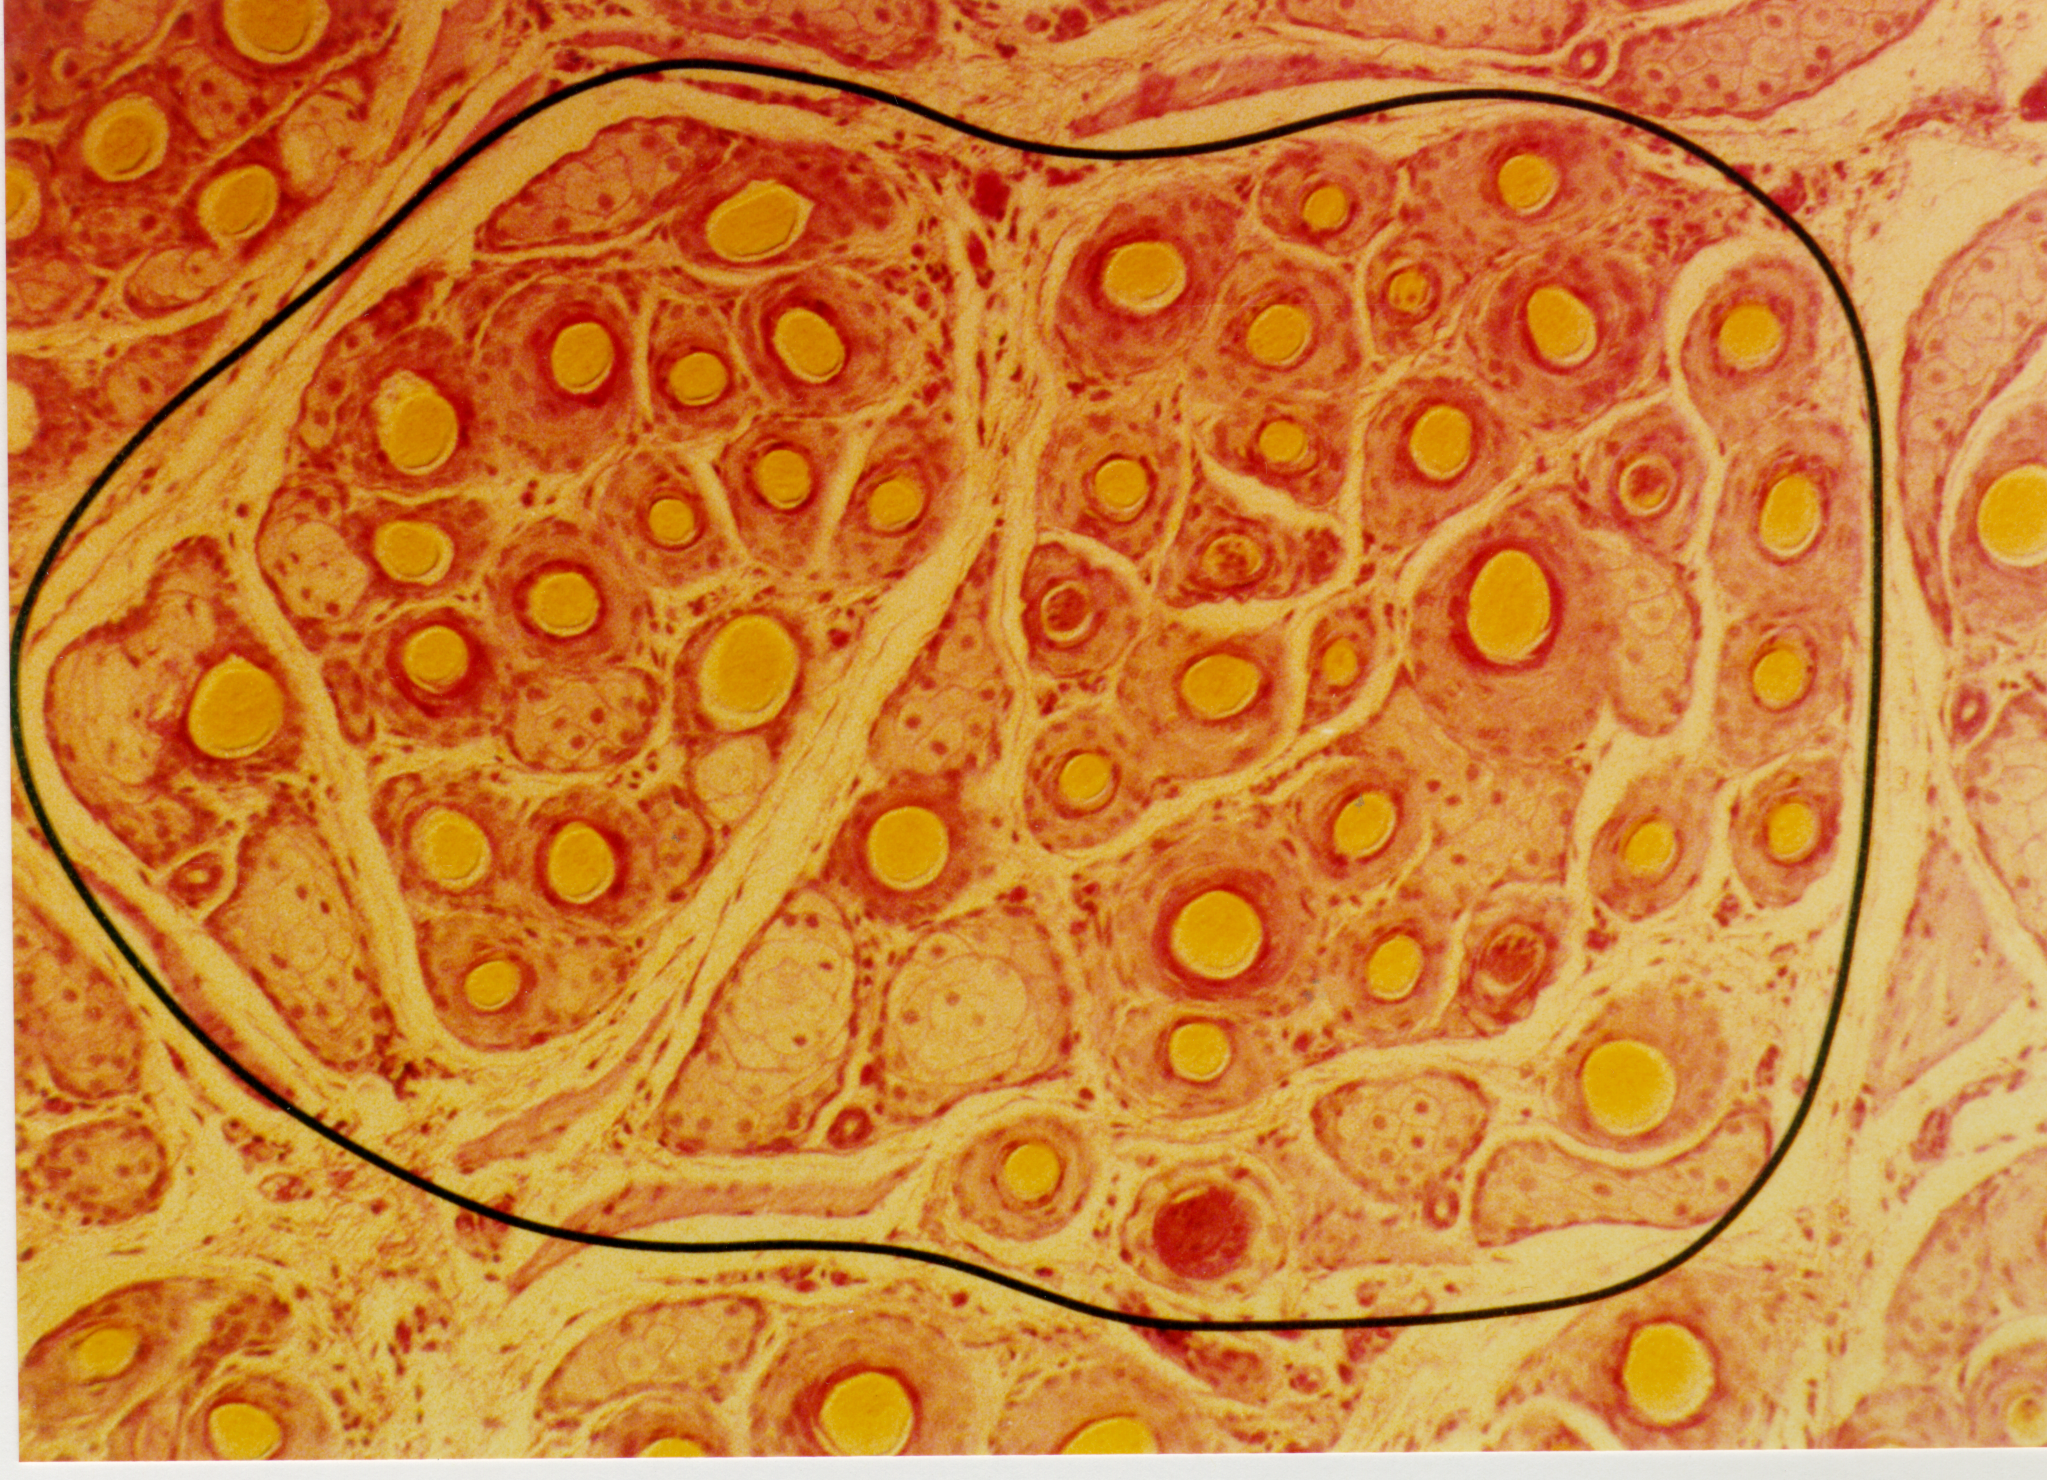
\includegraphics[width=\textwidth, trim = 0 20 0 120]{images/fig14a.png}
  }
  \subfigure[Plate (ii) x... magnification.]{
    \label{fig:14(ii)}
    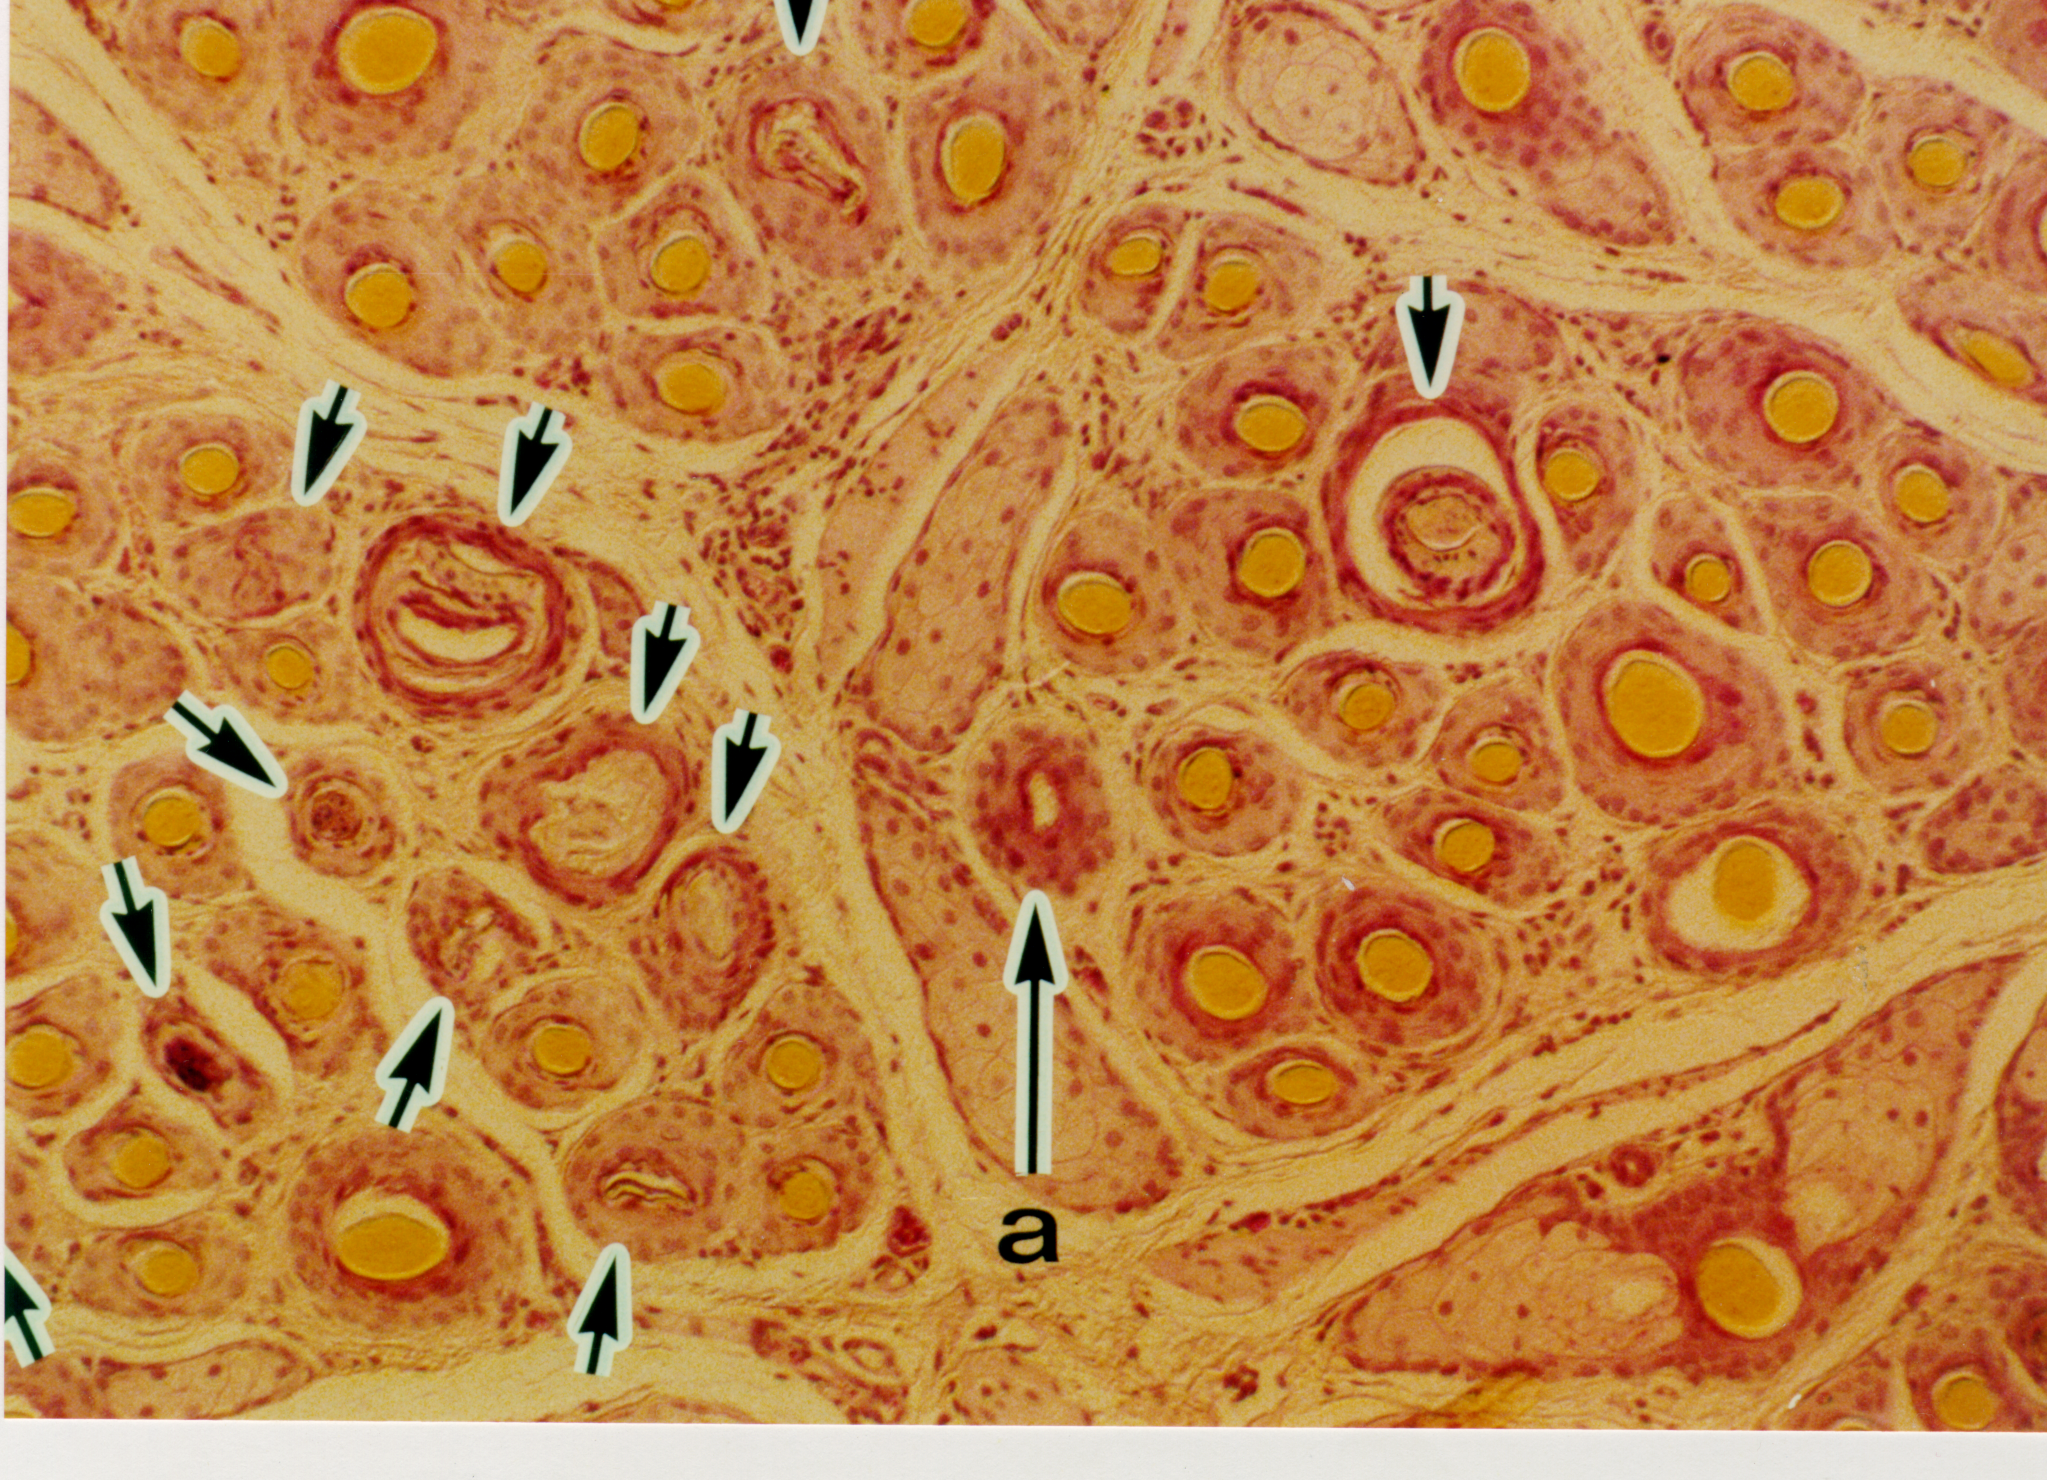
\includegraphics[width=\textwidth, trim = 0 20 0 20]{images/fig14b.png}
  }
  \caption{ Transverse section of skin from the specimen of 
	 Figure~\ref{fig:13}.  Plate
         (i) shows a trio group with large primary and secondary fibres.
	  Plate (ii) shows (a) a shed primary follicle, and (b) all
          unlabelled arrows show secondary follicles in various stages of
	  shedding. }
  \label{fig:14}
\end{figure}

%\end{document}
